\chapter{Methodology and Model Design}

The AquaTrack methodology combines laboratory prototype development with a computational prediction pipeline. Hydrogel patches are synthesized and evaluated for sweat collection and colorimetric response, while biomarker and context datasets are processed to train dehydration-risk classifiers. The design emphasizes modularity so that sensing, preprocessing, model training, fusion, and deployment can be improved independently.

\section{Hydrogel Synthesis}

Hydrogels are flexible polymer networks formed through extensive cross-linking between polymer chains. They can absorb and retain water, making them useful in biomedical applications such as wound dressing, drug delivery, implantable devices, and wearable biosensing. Two synthesis routes were evaluated in this work: sodium alginate hydrogel and polyvinyl alcohol hydrogel.

\subsection{Sodium Alginate Hydrogel}

Sodium alginate hydrogel was prepared by combining 2\% sodium alginate powder with distilled water. Glycerol was added as a plasticizer to improve flexibility and reduce folding during drying. The mixture was stirred at approximately 50--60$^\circ$C using a magnetic stirrer until uniform. After stirring, phenol red was added as the pH indicator.

The mixture was allowed to cool to room temperature before adding activated urease enzyme. Urease was prepared from urease-active meal by dissolving it in distilled water and collecting the yellow upper layer containing the enzyme. The cooled hydrogel mixture was cast onto clean, dry petri plates with a thickness of approximately 0.5--1 cm.

A 2\% calcium chloride solution was sprayed on the cast hydrogel and allowed to stand until a skin formed. The plates were then flooded with calcium chloride solution so that the hydrogel remained submerged. Calcium ions cross-linked the alginate chains by forming ionic bridges between carboxylate groups, producing the solid hydrogel network. After cross-linking, excess calcium chloride was removed and the hydrogels were washed three times with distilled water. The plates were covered with cling film with small holes and air-dried for 7--10 days until flexible patches were obtained.

\begin{figure}[htb]
\centering
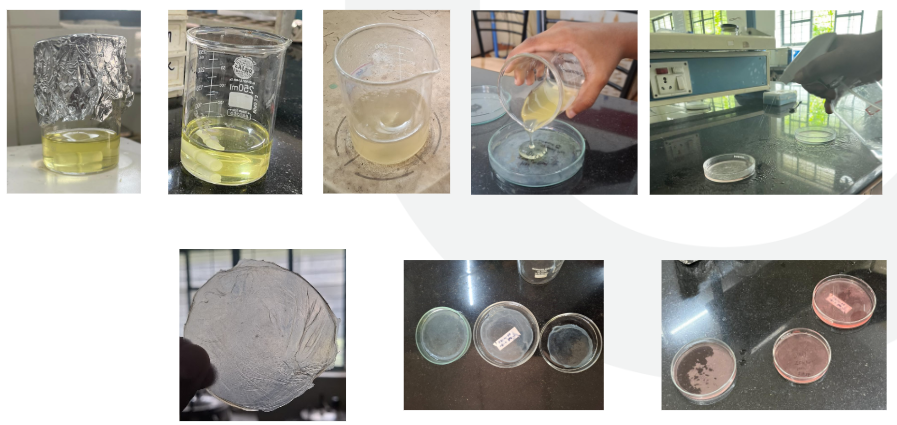
\includegraphics[width=0.9\textwidth]{Figures/aquatrack/image5}
\caption{Process of formation of sodium alginate hydrogel}
\label{fig:alginate-process}
\end{figure}

\subsection{Polyvinyl Alcohol Hydrogel}

Polyvinyl alcohol (PVA) hydrogels were synthesized using a cryogelation process. A mixture of 10\% PVA, distilled water, and glycerol was heated to approximately 80--90$^\circ$C. Phenol red was added after mixing, and activated urease was added only after cooling to protect enzyme activity. The mixture was poured into petri plates, sealed, and placed in a deep freezer at -20$^\circ$C overnight for the freeze cycle.

The samples were thawed at room temperature the next day. The freeze-thaw process was repeated three times over four days. During freezing, water crystallization pushes PVA chains closer together, promoting hydrogen bonding and crystallite formation. During thawing, the crystallites remain and create pores where water or sweat can enter. In the performed trials, PVA hydrogels did not cross-link successfully enough for use in the final prototype, so sodium alginate was selected.

\section{Dataset Description}

Two datasets were used for computational modeling. The main biomarker dataset, denoted as $D_{main}$, contains 90 observations from 10 healthy adult subjects measured across progressive running intervals. It contains 33 raw features across six modality groups: sweat biomarkers, salivary biomarkers, body composition and hydration, segmental bioelectrical impedance, peripheral skin temperature, and activity parameters.

The context dataset, denoted as $D_{ctx}$, contains 290 observations with 11 features measuring skin electrical properties, transepidermal water loss, ambient meteorological conditions, and time-of-day encoding.

\begin{table}[htb]
\fontsize{10}{12}\selectfont
\centering
\renewcommand{\arraystretch}{1.6}
\setlength{\extrarowheight}{4pt}
\caption{Dataset characteristics}
\label{tab:dataset-characteristics}
\begin{tabular}{|p{4cm}|p{4.2cm}|p{4.2cm}|}
\hline
\textbf{Property} & \textbf{Main Dataset ($D_{main}$)} & \textbf{Context Dataset ($D_{ctx}$)}\\
\hline
Total samples & 90 & 290\\
\hline
Raw features & 33 & 11\\
\hline
Target variable & dehydration\_risk (3-class) & dehydration\_label (binary)\\
\hline
Class balance & 30/30/30, quantile based & 50/50, balanced\\
\hline
\end{tabular}
\end{table}

\section{Target Engineering}

The biomarker dataset does not contain clinical ground-truth dehydration severity labels. Therefore, the target variable dehydration\_risk $\in$ \{Low, Medium, High\} is derived using a two-phase unsupervised learning procedure. A domain-weighted feature matrix is constructed by applying a 2$\times$ weight to primary biomarker features and a 0.5$\times$ weight to impedance features. K-Means clustering with $k=3$ is then applied.

Cluster labels are assigned using the composite rank score:
\begin{equation}
\label{eq:rank-score}
rank = \mu(Cl_{sw}) + \mu(Osm_{sw}) + \mu(Osm_{sal}) + \mu(Cl_{sal}) - \mu(TBW)
\end{equation}

Here, $\mu(\cdot)$ denotes the within-cluster mean. Higher sweat chloride, sweat osmolality, salivary osmolality, and salivary chloride indicate higher fluid depletion, while lower total body water indicates reduced hydration. The cluster with the lowest rank is assigned Low risk, the middle cluster Medium risk, and the highest cluster High risk.

\section{Preprocessing Pipeline}

\subsection{Median Imputation}

Missing values are concentrated in sweat and salivary marker columns. Column-wise median imputation is used because the data distribution is skewed and the mean could be inflated by extreme values. The median is computed only from the training partition within each cross-validation fold. For a feature $x$ with missing entries, the imputed value $\hat{x}_i$ is given by:
\begin{equation}
\label{eq:median-imputation}
\hat{x}_i = 
\begin{cases} 
x_i & \text{if } x_i \text{ is observed} \\
\text{median}(X_{train}) & \text{if } x_i \text{ is missing}
\end{cases}
\end{equation}

\subsection{Winsorization}

Extreme values in sweat and salivary biomarker columns are handled through winsorization. Observations exceeding the selected boundary are clipped to the fence value rather than deleted. A 3$\times$ IQR boundary is used because skewed distributions can inflate standard deviation and reduce the reliability of z-score thresholds. The winsorized value $x'_i$ is defined as:
\begin{equation}
\label{eq:winsorization}
x'_i = 
\begin{cases} 
Q_1 - 3 \times IQR & \text{if } x_i < Q_1 - 3 \times IQR \\
Q_3 + 3 \times IQR & \text{if } x_i > Q_3 + 3 \times IQR \\
x_i & \text{otherwise}
\end{cases}
\end{equation}
where $IQR = Q_3 - Q_1$.

\subsection{Logarithmic Transformation}

Logarithmic transformation compresses large values in skewed distributions and stabilizes variance. Five biomarker features receive a $\log(1+x)$ transformation: salivary protein concentration, salivary amylase, salivary cortisol, salivary potassium, and salivary osmolality. The transformation is expressed as:
\begin{equation}
\label{eq:log-transform}
x_{log} = \ln(1 + x)
\end{equation}

\subsection{Robust Scaling Normalization}

Robust scaling uses the median and interquartile range instead of the mean and standard deviation. This makes it resistant to outliers. All features in both pipelines are normalized using robust scaling after imputation, winsorization, and transformation. The scaled value $x_{robust}$ is calculated as:
\begin{equation}
\label{eq:robust-scaling}
x_{robust} = \frac{x - \text{median}(X)}{Q_3(X) - Q_1(X)}
\end{equation}

\section{Feature Extraction and Selection}

To bridge the gap between raw sensor data and latent states, a domain-driven feature engineering strategy is employed. Feature extraction is designed to reduce multicollinearity and synthesize clinically meaningful representations of hydration status. Interaction-aware feature representations are constructed by consolidating highly correlated variables into composite indices, thereby ensuring dimensional optimization without loss of predictive relevance. These are detailed in Table \ref{tab:feature-descriptions}. Following the synthesis of engineered features, an embedded feature selection mechanism is implemented to identify the most discriminative variables for each pipeline.

\begin{table}[htb]
\fontsize{10}{12}\selectfont
\centering
\renewcommand{\arraystretch}{1.6}
\setlength{\extrarowheight}{4pt}
\caption{Selected feature descriptions}
\label{tab:feature-descriptions}
\begin{tabular}{|p{3.4cm}|p{3.8cm}|p{4.4cm}|p{2.2cm}|}
\hline
\textbf{\makecell[l]{Engineered\\ Feature}} & \textbf{Formula} & \textbf{Clinical Rationale} & \textbf{Pipeline}\\
\hline
Sweat Stress Index & $Cl_{sw} + Osm_{sw}$ & Combines correlated sweat markers & Main\\
\hline
Saliva Dehydration Index & $Osm_{sal} + Cl_{sal}$ & Combines correlated salivary markers & Main\\
\hline
Hydration Ratio & $TBW/body\_weight$ & Normalizes the whole-body water for body size & Main\\
\hline
Exertion Load & $speed \times interval$ & Quantifies cumulative exercise-induced stress & Main\\
\hline
Skin Hydration Index & \makecell[l]{$Capacitance/$ \\ $(Impedance/1000)$} & Amplifies the skin hydration signal & Context\\
\hline
Environmental Stress Index & $T_{amb} \times (1 - RH/100)$ & Represents hot and dry environmental demand & Context\\
\hline
Skin Stress Score & $TEWL \times T_{skin}$ & Combines barrier loss and skin temperature & Context\\
\hline
\end{tabular}
\end{table}

\section{Model Training, Selection and Evaluation}

The prediction engine evaluates four distinct classifier families: Logistic Regression (LR), Random Forest (RF), RBF-kernel Support Vector Machine (SVM), and Gradient Boosting. Hyperparameter optimization is performed using GridSearchCV over extensive search spaces, including regularization penalties, tree depth, and kernel bandwidth. Model selection is guided by stratified 10-fold cross-validation to ensure that each fold maintains the class distribution of the original dataset. The overall model construction and weighted fusion logic is formalized in Algorithm \ref{alg:fusion-procedure}. 
The comprehensive training configuration and specific hyperparameter search grids used for optimization 
are detailed in Table \ref{tab:training-config} and Table \ref{tab:hyperparameter-grid}, respectively.

\begin{algorithm}
\caption{Dual-pipeline model building and weighted fusion procedure}
\label{alg:fusion-procedure}
\begin{algorithmic}[1]
\State \textbf{Input:} $D_{main}$ with selected biomarker features, $D_{ctx}$ with selected context features
\State \textbf{Output:} fused score $F \in [0,1]$, risk label $\in$ \{Low, Medium, High\}, consistency flag
\State Prepare $X_m, y_m$ from $D_{main}$ and perform stratified train-test split.
\State Train Logistic Regression, Random Forest, SVM, and Gradient Boosting with robust scaling and balanced class weighting.
\State Select the best biomarker classifier using 10-fold cross-validation and macro F1 score.
\State Evaluate the selected biomarker model once on the held-out test set.
\State Prepare $X_c, y_c$ from $D_{ctx}$ and repeat model selection using binary F1 score.
\State Compute $S_{main}$ and $S_{ctx}$ from the selected model probabilities.
\State Compute $F = 0.6 \times S_{main} + 0.4 \times S_{ctx}$.
\State Flag conflicts when the categorical prediction and weighted fused score disagree beyond threshold limits.
\end{algorithmic}
\end{algorithm}

\clearpage

\begin{table}[ht]
\small
\centering
\caption{Training configuration and design decisions applied in both pipelines.}
\label{tab:training-config}
\begin{tabular}{lll}
\toprule
\textbf{Component} & \textbf{Decision} & \textbf{Justification} \\
\midrule
Train-Test Split & 80/20 stratified & Preserves class balance in both partitions \\
Cross-Validation & 10-Fold StratifiedKFold & Maximises training data per fold at n=90 \\
Scoring Metric & Macro F1 & Equal class importance regardless of size \\
Class Handling & class\_weight=balanced & Prevents majority-class dominance \\
Scaling & RobustScaler (in Pipeline) & Outlier-resistant, leakage-free \\
Hyperparameter Search & GridSearchCV & Exhaustive search over defined grids \\
Model Selection & Best CV Macro F1 on train & Test set never used for selection \\
Test Evaluation & Once, post-selection only & Prevents selection bias \\
\bottomrule
\end{tabular}
\end{table}

\begin{table}[ht]
\small
\centering
\caption{Hyperparameter tuning search grids used in GridSearchCV}
\label{tab:hyperparameter-grid}
\begin{tabular}{lll}
\toprule
\textbf{Classifier} & \textbf{Parameter} & \textbf{Values Searched} \\
\midrule
\multirow{3}{*}{Logistic Regression} & C & 0.01, 0.1, 1, 10 \\
& solver & lbfgs, saga \\
& max\_iter & 1000 (fixed) \\
\midrule
\multirow{3}{*}{Random Forest} & n\_estimators & 50, 100, 200 \\
& max\_depth & None, 5, 10 \\
& min\_samples\_leaf & 1, 2 \\
\midrule
\multirow{2}{*}{SVM (RBF)} & C & 0.1, 1, 10 \\
& gamma & scale, auto \\
\midrule
\multirow{3}{*}{Gradient Boosting} & n\_estimators & 50, 100 \\
& learning\_rate & 0.05, 0.1 \\
& max\_depth & 3, 5 \\
\bottomrule
\end{tabular}
\end{table}
